\section{lib/efreet\_\-icon.c File Reference}
\label{efreet__icon_8c}\index{lib/efreet\_\-icon.c@{lib/efreet\_\-icon.c}}


{\tt \#include \char`\"{}Efreet.h\char`\"{}}\par
{\tt \#include \char`\"{}efreet\_\-private.h\char`\"{}}\par


Include dependency graph for efreet\_\-icon.c:\nopagebreak
\begin{figure}[H]
\begin{center}
\leavevmode
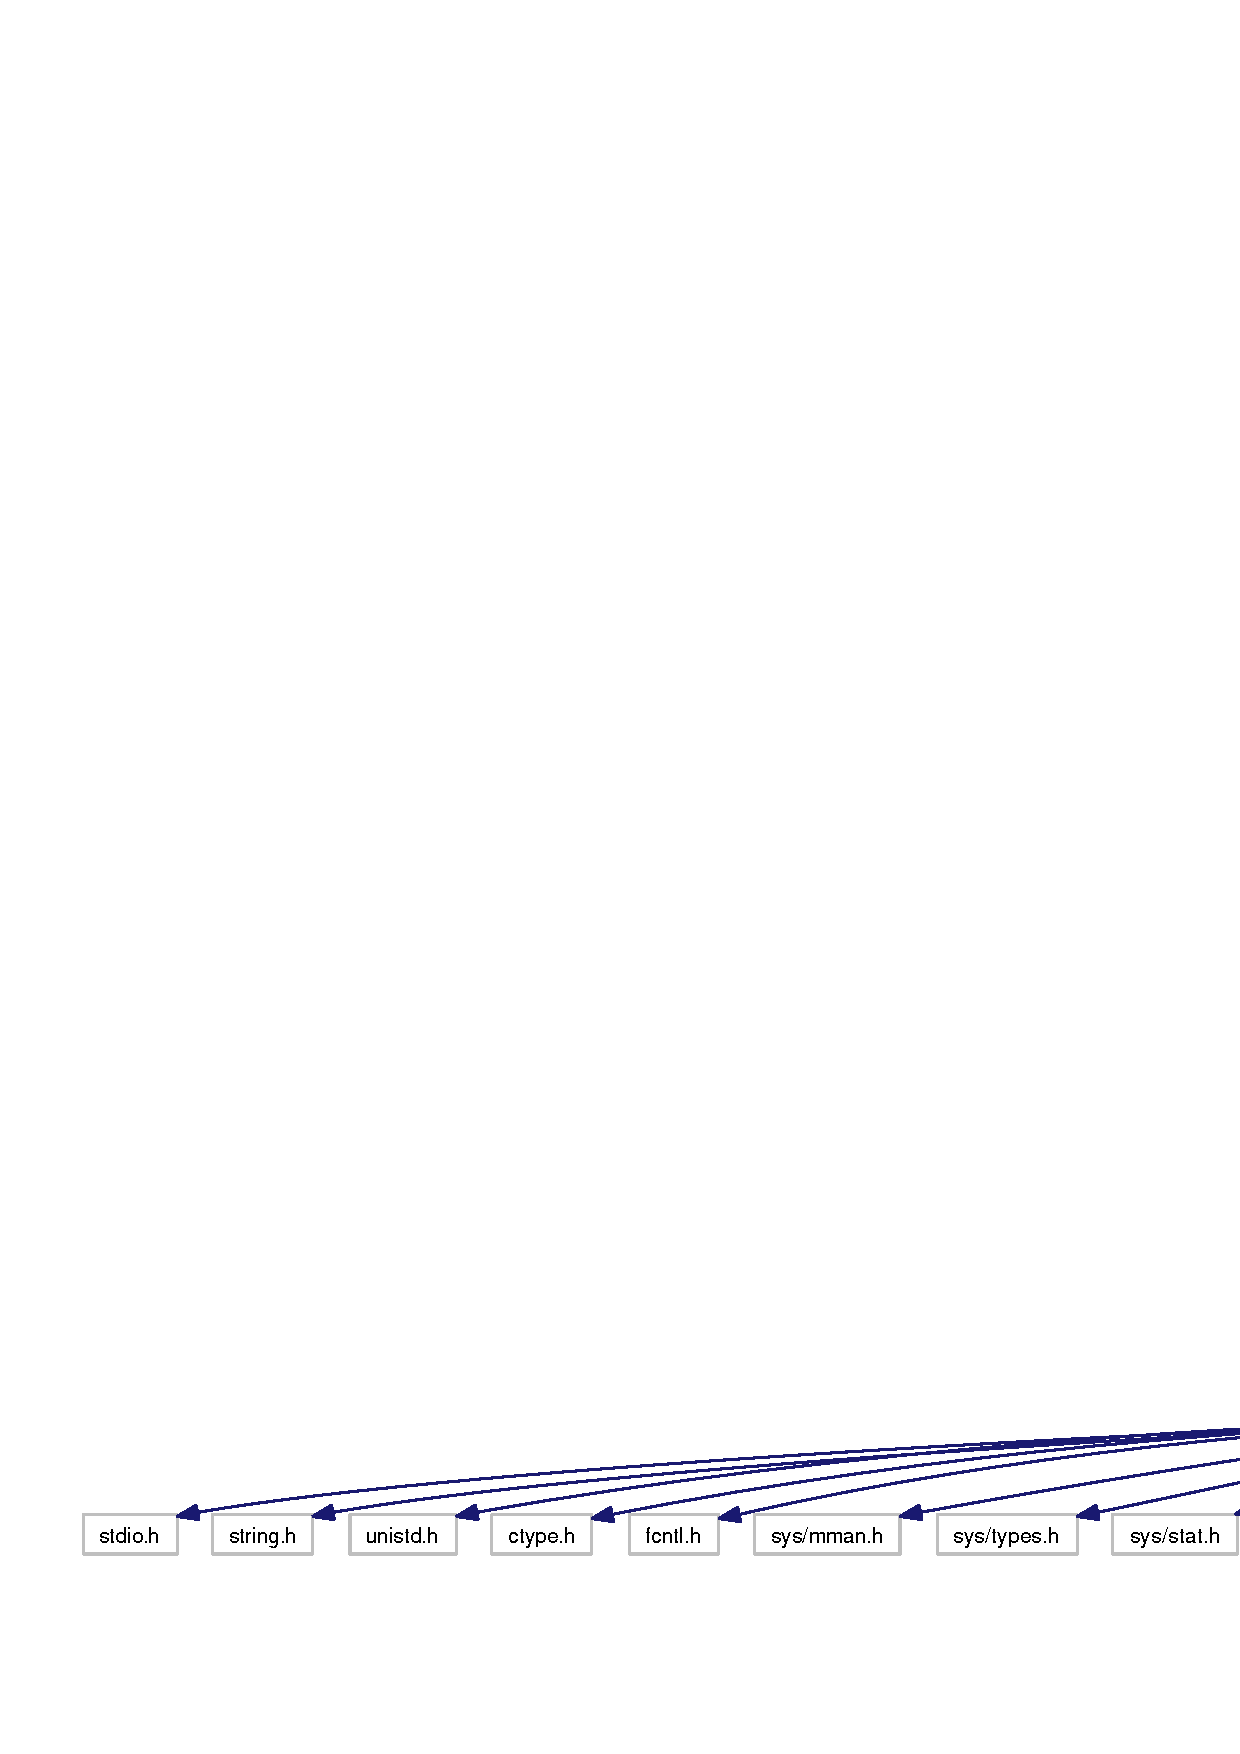
\includegraphics[width=420pt]{efreet__icon_8c__incl}
\end{center}
\end{figure}
\subsection*{Data Structures}
\begin{CompactItemize}
\item 
struct {\bf Efreet\_\-Icon\_\-Cache}
\end{CompactItemize}
\subsection*{Defines}
\begin{CompactItemize}
\item 
\#define {\bf NON\_\-EXISTING}~(void $\ast$)-1
\end{CompactItemize}
\subsection*{Typedefs}
\begin{CompactItemize}
\item 
typedef struct {\bf Efreet\_\-Icon\_\-Cache} {\bf Efreet\_\-Icon\_\-Cache}
\end{CompactItemize}
\subsection*{Functions}
\begin{CompactItemize}
\item 
const char $\ast$ {\bf efreet\_\-icon\_\-deprecated\_\-user\_\-dir\_\-get} (void)
\begin{CompactList}\small\item\em Returns the user icon directory. \item\end{CompactList}\item 
EAPI void {\bf efreet\_\-icon\_\-extension\_\-add} (const char $\ast$ext)
\begin{CompactList}\small\item\em Adds the given extension to the list of possible icon extensions. \item\end{CompactList}\item 
EAPI Ecore\_\-List $\ast$ {\bf efreet\_\-icon\_\-extra\_\-list\_\-get} (void)
\begin{CompactList}\small\item\em Gets the list of all extra directories to look for icons. These directories are used to look for icons after looking in the user icon dir and before looking in standard system directories. The order of search is from first to last directory in this list. the strings in the list should be created with eina\_\-stringshare\_\-add(). \item\end{CompactList}\item 
EAPI {\bf Efreet\_\-Icon} $\ast$ {\bf efreet\_\-icon\_\-find} (const char $\ast$theme\_\-name, const char $\ast$icon, unsigned int size)
\begin{CompactList}\small\item\em Retrieves all of the information about the given icon. \item\end{CompactList}\item 
EAPI void {\bf efreet\_\-icon\_\-free} ({\bf Efreet\_\-Icon} $\ast$icon)
\begin{CompactList}\small\item\em Free's the given icon and all its internal data. \item\end{CompactList}\item 
int {\bf efreet\_\-icon\_\-init} (void)
\item 
EAPI char $\ast$ {\bf efreet\_\-icon\_\-list\_\-find} (const char $\ast$theme\_\-name, Ecore\_\-List $\ast$icons, unsigned int size)
\begin{CompactList}\small\item\em Retrieves all of the information about the first found icon in the list. \item\end{CompactList}\item 
EAPI char $\ast$ {\bf efreet\_\-icon\_\-path\_\-find} (const char $\ast$theme\_\-name, const char $\ast$icon, unsigned int size)
\begin{CompactList}\small\item\em Retrives the path to the given icon. \item\end{CompactList}\item 
void {\bf efreet\_\-icon\_\-shutdown} (void)
\item 
EAPI {\bf Efreet\_\-Icon\_\-Theme} $\ast$ {\bf efreet\_\-icon\_\-theme\_\-find} (const char $\ast$theme\_\-name)
\begin{CompactList}\small\item\em Tries to get the icon theme structure for the given theme name. \item\end{CompactList}\item 
EAPI Ecore\_\-List $\ast$ {\bf efreet\_\-icon\_\-theme\_\-list\_\-get} (void)
\begin{CompactList}\small\item\em Retrieves all of the non-hidden icon themes available on the system. The returned list must be freed. Do not free the list data. \item\end{CompactList}\item 
EAPI const char $\ast$ {\bf efreet\_\-icon\_\-user\_\-dir\_\-get} (void)
\end{CompactItemize}


\subsection{Define Documentation}
\index{efreet\_\-icon.c@{efreet\_\-icon.c}!NON\_\-EXISTING@{NON\_\-EXISTING}}
\index{NON\_\-EXISTING@{NON\_\-EXISTING}!efreet_icon.c@{efreet\_\-icon.c}}
\subsubsection[NON\_\-EXISTING]{\setlength{\rightskip}{0pt plus 5cm}\#define NON\_\-EXISTING~(void $\ast$)-1}\label{efreet__icon_8c_3da87339a2ab67dd100b8fc9efa92247}




Referenced by efreet\_\-icon\_\-list\_\-find(), and efreet\_\-icon\_\-path\_\-find().

\subsection{Typedef Documentation}
\index{efreet\_\-icon.c@{efreet\_\-icon.c}!Efreet\_\-Icon\_\-Cache@{Efreet\_\-Icon\_\-Cache}}
\index{Efreet\_\-Icon\_\-Cache@{Efreet\_\-Icon\_\-Cache}!efreet_icon.c@{efreet\_\-icon.c}}
\subsubsection[Efreet\_\-Icon\_\-Cache]{\setlength{\rightskip}{0pt plus 5cm}typedef struct {\bf Efreet\_\-Icon\_\-Cache} {\bf Efreet\_\-Icon\_\-Cache}}\label{efreet__icon_8c_357003192381c449f058fd0380580be7}




\subsection{Function Documentation}
\index{efreet\_\-icon.c@{efreet\_\-icon.c}!efreet\_\-icon\_\-deprecated\_\-user\_\-dir\_\-get@{efreet\_\-icon\_\-deprecated\_\-user\_\-dir\_\-get}}
\index{efreet\_\-icon\_\-deprecated\_\-user\_\-dir\_\-get@{efreet\_\-icon\_\-deprecated\_\-user\_\-dir\_\-get}!efreet_icon.c@{efreet\_\-icon.c}}
\subsubsection[efreet\_\-icon\_\-deprecated\_\-user\_\-dir\_\-get]{\setlength{\rightskip}{0pt plus 5cm}const char$\ast$ efreet\_\-icon\_\-deprecated\_\-user\_\-dir\_\-get (void)}\label{efreet__icon_8c_cc8dbdb67b18a402ac80b3121bb590e5}


Returns the user icon directory. 

\begin{Desc}
\item[Returns:]Returns the user icon directory \end{Desc}


References efreet\_\-home\_\-dir\_\-get().